\documentclass[12pt]{article}
\usepackage{graphicx}
\usepackage{geometry}
\usepackage{fancyhdr}
\usepackage{titletoc}
\usepackage{titlesec}
\usepackage{listings}
\usepackage{booktabs}
\usepackage{adjustbox} % Add this line

% Page setup
\geometry{
    top=1in,
    bottom=1in,
    left=1in, % Adjust the left margin
    right=1in, % Adjust the right margin
}

% breaklines=true,

\pagestyle{fancy}
\fancyhf{} % Clear all header and footer fields
\fancyhead[R]{Evolutionary Algorithms} % Add this line to set the header on the right side
\renewcommand{\headrulewidth}{0pt} % Remove the horizontal line in the header

% Define section numbering format
\titleformat{\section}{\normalfont\large\bfseries}{\thesection}{1em}{}
\titleformat{\subsection}{\normalfont\normalsize\bfseries}{\thesubsection}{1em}{}

% Title Page
\begin{document}
\begin{titlepage}
    \centering
    {\LARGE\textbf{CS 451 : Computational Intelligence}\par}
    \vspace{0.5cm}
    {\Large Assignment 1\par}
    \vspace{0.2cm}
    {\Large Evolutionary Algorithms\par}
    \vspace*{\fill} % Vertically center the logo and text
    {\large Mustafa Sohail $\mid$ ms06860@st.habib.edu.pk\par}
    {\large Muhammad Azeem Haider $\mid$ mh06858@st.habib.edu.pk\par}
    \vspace{2cm}
    
\includegraphics[height=7cm]{images/HU_logo}\\\bigskip
    {\large \today}\\\bigskip\bigskip
    \vspace{1cm}
    \vspace{2cm}
    {\large Dhanani School of Science and Engineering\par}
    {\large Habib University\par}
    {\large Spring 2024\par}
    \vspace*{\fill} % Vertically center the copyright text
    % {\large Copyright @ 2024 Habib University\par}
\end{titlepage}

% Index page
\thispagestyle{empty} % No page number on index page
\tableofcontents
\clearpage

\section{Introduction}
The first assignment of the course Computational Intelligence (CS-451) required us to implement evolutionary algorithms for three problems which are as followed:

\begin{enumerate}
    \item \textbf{Travelling Salesman Problem:} The Travelling Salesman Problem (TSP) is a classic problem in combinatorial optimization. It is the problem of finding a tour of a set of n cities that is of minimum cost. A tour is a permutation of the cities, and the cost of a tour is the sum of the distances between adjacent cities in the tour.
    \item \textbf{Job-Shop Scheduling Problem:} The job-shop scheduling problem is a classic problem in combinatorial optimization. It is the problem of scheduling a set of n jobs on a set of m machines. Each job consists of a sequence of operations, each of which must be processed on a specific machine for a specific amount of time.
    \item \textbf{Evolutionary Art (Mona Lisa):} The evolutionary art problem is a classic problem in evolutionary computation. It is the problem of evolving a population of images to match a target image. Each image in the population is represented as a string of genes, and the fitness of an image is the similarity between the image and the target image.
\end{enumerate}

\section{Travelling Salesman Problem}

\subsection{Problem Formulation}

The travelling salesman problem requires finding of the minimum cost (distance) to cover all the cities. The \textbf{chromosome generation} is being carried out by randomly shuffling the cities of the Qatar dataset. 
\newline \\
Furthermore, the \textbf{mutate function} assigns each chromosome a random number from 0 to 1, and if the number is less than the mutation rate, mutation occurs. 
\newline \\
Finally, the \textbf{crossover function} once again, carries out crossover between two parents by assigning the crossover point, and all the repeated cities from the second parent, that are already added in the first part, are added linearly in the end. 

\subsection{Analysis}

While carrying out initial combination for selection schemes for parent selection and survival selection, it was clear that a combination of an explorative scheme as a parent selection and an exploitative scheme as a survival selection would be the best. As a result, the main combinations that were tested were the following:

    \begin{itemize}
        \item \textbf{Parent Selection:} Random \textbf{Survival Selection:} truncation
    \end{itemize}

% We yeilded the following result for the first combination, where we had two extremes as the parent selection and survival selection schemes:
Our best score for TSP was just under 17500. The result reported in \textit{Figure 1}, was obtained by the following parameters:


% \begin{center}
\begin{figure}[h]
    \centering
    \includegraphics[width=0.5\textwidth]{images/figure_1.png}
    \caption{TSP - Best score graph}
\end{figure}
% \end{center}

% \newpage

\begin{enumerate}
    \item \textbf{Population Size:} 1000
    \item \textbf{Offspring Size:} 200
    \item \textbf{Number of Generations:} 5000
    \item \textbf{Mutation Rate:} 0.45
    \item \textbf{Iterations:} 10
\end{enumerate}

The following graph Figure 2, has the same selection schemes and parameters, except for the fact that it is ran on 25 generations, to attach statistics for the Best Fitness and Average Fitness.

\begin{figure}[h]
    \centering
    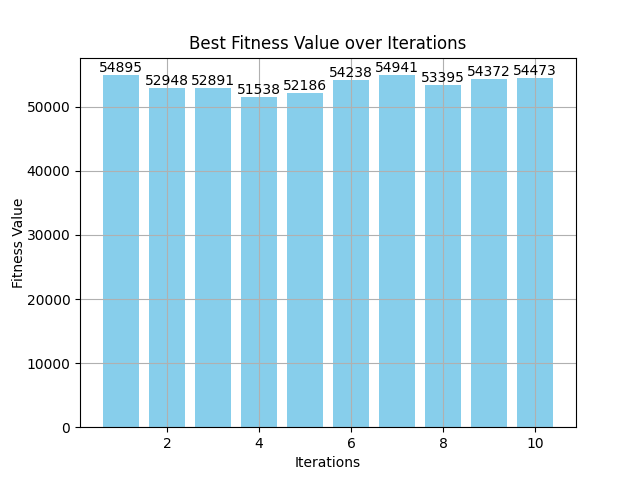
\includegraphics[width=0.5\textwidth]{images/TSPlessgen.png}
    \caption{TSP - Best score graph with fewer generations}
\end{figure}

\begin{table}[h]
    \centering
    \caption{Best Fitness Score Across generations for 10 iterations}
    \label{tab:fitness_scores}
    \begin{adjustbox}{max width=0.7\textwidth} % Adjust the table width
        \begin{tabular}{*{12}{c}}
            \toprule
            Generations & Iteration 1 & Iteration 2 & Iteration 3 & Iteration 4 & Iteration 5 & Iteration 6 & Iteration 7 & Iteration 8 & Iteration 9 & Iteration 10 & Best Fitness Score \\
            \midrule
            Gen 1 & 82057 & 83328 & 85114 & 83051 & 82434 & 84352 & 84152 & 83083 & 85161 & 85063 & 82057 \\
            Gen 2 & 72757 & 71186 & 72579 & 72855 & 72946 & 73058 & 72463 & 73370 & 73611 & 73278 & 71186 \\
            Gen 3 & 69428 & 66881 & 66965 & 66927 & 65977 & 70057 & 70021 & 67938 & 69691 & 67122 & 65977 \\
            Gen 4 & 67481 & 64362 & 66965 & 66927 & 64392 & 68479 & 64360 & 66363 & 64316 & 66668 & 64316 \\
            Gen 5 & 64840 & 64362 & 65886 & 61476 & 62560 & 64157 & 64360 & 65278 & 64311 & 64785 & 61476 \\
            Gen 6 & 62950 & 63512 & 64510 & 61476 & 62560 & 63938 & 64360 & 64894 & 64311 & 64785 & 61476 \\
            Gen 7 & 62950 & 63512 & 61883 & 61476 & 62147 & 62418 & 62384 & 63854 & 60865 & 63241 & 60865 \\
            Gen 8 & 61595 & 60080 & 61358 & 61398 & 61788 & 60598 & 62103 & 61661 & 60865 & 59061 & 59061 \\
            Gen 9 & 61595 & 60080 & 61358 & 59119 & 60343 & 60598 & 61586 & 60238 & 60865 & 59061 & 59061 \\
            Gen 10 & 60322 & 60080 & 60330 & 56919 & 60062 & 60598 & 60953 & 60238 & 60865 & 59061 & 56919 \\
            Gen 11 & 58853 & 59368 & 58523 & 56919 & 55649 & 59813 & 57890 & 58235 & 58962 & 56718 & 55649 \\
            Gen 12 & 58853 & 58297 & 58523 & 56919 & 55649 & 59232 & 56851 & 58235 & 58962 & 56718 & 55649 \\
            Gen 13 & 58853 & 57651 & 58523 & 56919 & 55649 & 59232 & 56851 & 57703 & 56276 & 56718 & 55649 \\
            Gen 14 & 58523 & 57651 & 58135 & 55778 & 55649 & 59232 & 56851 & 57703 & 56276 & 56718 & 55649 \\
            Gen 15 & 57789 & 56022 & 58135 & 55778 & 55638 & 57492 & 56851 & 57703 & 56276 & 56343 & 55638 \\
            Gen 16 & 57789 & 55946 & 55068 & 55778 & 55638 & 57234 & 56851 & 55921 & 56276 & 55681 & 55068 \\
            Gen 17 & 55403 & 55946 & 55068 & 55778 & 55638 & 56635 & 56851 & 55921 & 56276 & 55681 & 55068 \\
            Gen 18 & 55403 & 55946 & 54933 & 55008 & 55638 & 56187 & 56851 & 55921 & 56276 & 55681 & 54933 \\
            Gen 19 & 55403 & 55946 & 54933 & 54031 & 55422 & 56187 & 56851 & 55921 & 54689 & 55681 & 54031 \\
            Gen 20 & 55403 & 52948 & 54712 & 51538 & 54981 & 55864 & 56447 & 55921 & 54689 & 54883 & 51538 \\
            Gen 21 & 54895 & 52948 & 52891 & 51538 & 54934 & 55864 & 56447 & 53395 & 54689 & 54883 & 51538 \\
            Gen 22 & 54895 & 52948 & 52891 & 51538 & 54934 & 55864 & 56015 & 53395 & 54689 & 54859 & 51538 \\
            Gen 23 & 54895 & 52948 & 52891 & 51538 & 54934 & 55503 & 56015 & 53395 & 54689 & 54859 & 51538 \\
            Gen 24 & 54895 & 52948 & 52891 & 51538 & 54934 & 54710 & 55802 & 53395 & 54689 & 54754 & 51538 \\
            Gen 25 & 54895 & 52948 & 52891 & 51538 & 54678 & 54710 & 55802 & 53395 & 54689 & 54754 & 51538 \\
            \bottomrule
        \end{tabular}
    \end{adjustbox}
\end{table}

\begin{table}[h]
    \centering
    \caption{Average Fitness Scores Across generations for 10 iterations}
    \label{tab:fitness_scores}
    \begin{adjustbox}{max width=0.7\textwidth} % Adjust the table width
        \begin{tabular}{*{12}{c}}
            \toprule
            Generations & Iteration 1 & Iteration 2 & Iteration 3 & Iteration 4 & Iteration 5 & Iteration 6 & Iteration 7 & Iteration 8 & Iteration 9 & Iteration 10 & Average Fitness Score \\
            \midrule
            Gen 1 & 82057 & 83328 & 85114 & 83051 & 82434 & 84352 & 84152 & 83083 & 85161 & 85063 & 83660 \\
            Gen 2 & 72757 & 71186 & 72579 & 72855 & 72946 & 73058 & 72463 & 73370 & 73611 & 73278 & 72702 \\
            Gen 3 & 69428 & 66881 & 66965 & 66927 & 65977 & 70057 & 70021 & 67938 & 69691 & 67122 & 67829 \\
            Gen 4 & 67481 & 64362 & 66965 & 66927 & 64392 & 68479 & 64360 & 66363 & 64316 & 66668 & 65899 \\
            Gen 5 & 64840 & 64362 & 65886 & 61476 & 62560 & 64157 & 64360 & 65278 & 64311 & 64785 & 63937 \\
            Gen 6 & 62950 & 63512 & 64510 & 61476 & 62560 & 63938 & 64360 & 64894 & 64311 & 64785 & 63695 \\
            Gen 7 & 62950 & 63512 & 61883 & 61476 & 62147 & 62418 & 62384 & 63854 & 60865 & 63241 & 62561 \\
            Gen 8 & 61595 & 60080 & 61358 & 61398 & 61788 & 60598 & 62103 & 61661 & 60865 & 59061 & 60999 \\
            Gen 9 & 61595 & 60080 & 61358 & 59119 & 60343 & 60598 & 61586 & 60238 & 60865 & 59061 & 60595 \\
            Gen 10 & 60322 & 60080 & 60330 & 56919 & 60062 & 60598 & 60953 & 60238 & 60865 & 59061 & 59570 \\
            Gen 11 & 58853 & 59368 & 58523 & 56919 & 55649 & 59813 & 57890 & 58235 & 58962 & 56718 & 58073 \\
            Gen 12 & 58853 & 58297 & 58523 & 56919 & 55649 & 59232 & 56851 & 58235 & 58962 & 56718 & 58050 \\
            Gen 13 & 58853 & 57651 & 58523 & 56919 & 55649 & 59232 & 56851 & 57703 & 56276 & 56718 & 57897 \\
            Gen 14 & 58523 & 57651 & 58135 & 55778 & 55649 & 59232 & 56851 & 57703 & 56276 & 56718 & 57781 \\
            Gen 15 & 57789 & 56022 & 58135 & 55778 & 55638 & 57492 & 56851 & 57703 & 56276 & 56343 & 57021 \\
            Gen 16 & 57789 & 55946 & 55068 & 55778 & 55638 & 57234 & 56851 & 55921 & 56276 & 55681 & 56342 \\
            Gen 17 & 55403 & 55946 & 55068 & 55778 & 55638 & 56635 & 56851 & 55921 & 56276 & 55681 & 56175 \\
            Gen 18 & 55403 & 55946 & 54933 & 55008 & 55638 & 56187 & 56851 & 55921 & 56276 & 55681 & 55918 \\
            Gen 19 & 55403 & 55946 & 54933 & 54031 & 55422 & 56187 & 56851 & 55921 & 54689 & 55681 & 55577 \\
            Gen 20 & 55403 & 52948 & 54712 & 51538 & 54981 & 55864 & 56447 & 55921 & 54689 & 54883 & 54728 \\
            Gen 21 & 54895 & 52948 & 52891 & 51538 & 54934 & 55864 & 56447 & 53395 & 54689 & 54883 & 54323 \\
            Gen 22 & 54895 & 52948 & 52891 & 51538 & 54934 & 55864 & 56015 & 53395 & 54689 & 54859 & 54120 \\
            Gen 23 & 54895 & 52948 & 52891 & 51538 & 54934 & 55503 & 56015 & 53395 & 54689 & 54859 & 53844 \\
            Gen 24 & 54895 & 52948 & 52891 & 51538 & 54934 & 54710 & 55802 & 53395 & 54689 & 54754 & 53645 \\
            Gen 25 & 54895 & 52948 & 52891 & 51538 & 54678 & 54710 & 55802 & 53395 & 54689 & 54754 & 53456 \\
            \bottomrule
        \end{tabular}
    \end{adjustbox}
\end{table}

\section{Job-Shop Scheduling Problem}

\subsection{Problem Formulation}

The job-shop scheduling problem requires finding the minimum time to complete all the jobs on all the machines.
\\ \newline
The chromosome is generated by providing each job with an index, and repeating that number of index for the number of operations on that job. For example for abz5, if there are 10 jobs with 10 operations each, each job will be given an index from 0-9 and each number from 0-9 will repeat exactly 10 times. In this manner, we have flattened our chromosome. 
\\ \newline
The mutate and crossover function work in similar fashion to the travelling salesman problem. The mutate function checks probability assigned and if it is less than mutation rate, mutation occurs, and crossover occurs between two parents, and repeated jobs from parent two are added in the end of the new offsprings. 

\subsection{Analysis}

Unlike, the travelling salesman problem, the job-shop scheduling problem had three input files which were abz(5-7). The analysis for each file will be divided into subsections.

\subsubsection{First input file ``abz5''}

The strategy to solve the job-shop scheduling problem was to use the same combination of parent selection and survival selection as the travelling salesman problem. Since keeping the parent selection scheme entirely explorative through \textit{random} function or on the higher exploration through rank-based selection or tournament selection. The survival selection was to be kept entirely exploitative through truncation or on the higher exploitation through fitness proportional selection. The best score achieved \textbf{1242} was through \textbf{random} and \textbf{truncation}, with the following parameters. 

\begin{enumerate}
    \item \textbf{Population Size:} 200
    \item \textbf{Offspring Size:} 60
    \item \textbf{Number of Generations:} 2000
    \item \textbf{Mutation Rate:} 0.5
    \item \textbf{Iterations:} 10
\end{enumerate}

\begin{figure}[h]
    \centering
    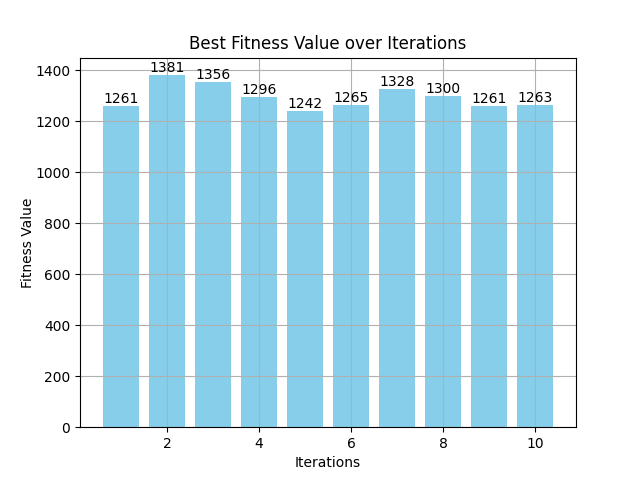
\includegraphics[width=0.5\textwidth]{images/Figure_2.png}
    \caption{JSSP - Best score graph}
\end{figure}

The following graph Figure 4, has the same selection schemes and parameters, except for the fact that it is ran on 25 generations, to attach statistics for the Best Fitness and Average Fitness.

\begin{figure}[h]
    \centering
    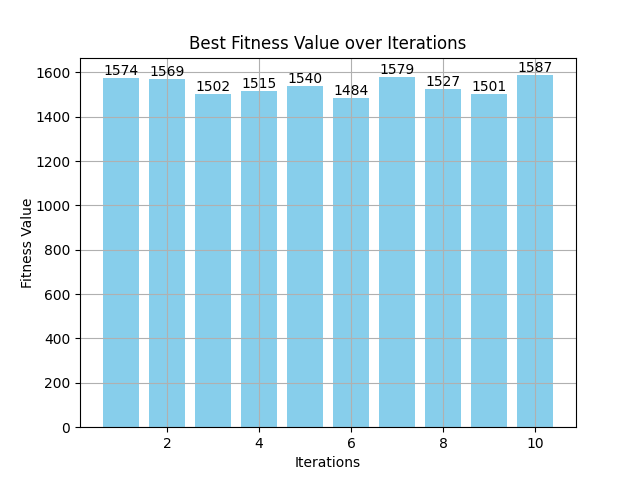
\includegraphics[width=0.45\textwidth]{images/JSSP_rntrbestscorelessgens.png}
    \caption{JSSP - Best score graph with fewer generations}
\end{figure}

Table 3 and 4 highlight the scores between the generations for 10 iterations, and the best and average scores amongst the generations. 

\newpage

\begin{table}[h]
    \centering
    \caption{Best Fitness Score Across generations for 10 iterations}
    \label{tab:fitness_scores}
    \begin{adjustbox}{max width=0.5\textwidth} % Adjust the table width
        \begin{tabular}{*{12}{c}}
        \toprule
        Generations & Iteration 1 & Iteration 2 & Iteration 3 & Iteration 4 & Iteration 5 & Iteration 6 & Iteration 7 & Iteration 8 & Iteration 9 & Iteration 10 & Best Fitness Score \\
        \midrule
        Gen 1 & 1718 & 1658 & 1741 & 1583 & 1640 & 1559 & 1656 & 1560 & 1533 & 1587 & 1533 \\
        Gen 2 & 1622 & 1658 & 1699 & 1583 & 1640 & 1559 & 1656 & 1560 & 1533 & 1587 & 1533 \\
        Gen 3 & 1622 & 1646 & 1699 & 1583 & 1640 & 1559 & 1656 & 1560 & 1533 & 1587 & 1533 \\
        Gen 4 & 1622 & 1646 & 1699 & 1583 & 1640 & 1559 & 1656 & 1560 & 1533 & 1587 & 1533 \\
        Gen 5 & 1622 & 1646 & 1699 & 1583 & 1640 & 1559 & 1656 & 1560 & 1533 & 1587 & 1533 \\
        Gen 6 & 1622 & 1632 & 1654 & 1583 & 1640 & 1559 & 1656 & 1560 & 1533 & 1587 & 1533 \\
        Gen 7 & 1622 & 1607 & 1631 & 1583 & 1640 & 1559 & 1656 & 1560 & 1533 & 1587 & 1533 \\
        Gen 8 & 1588 & 1593 & 1631 & 1551 & 1640 & 1559 & 1601 & 1560 & 1533 & 1587 & 1533 \\
        Gen 9 & 1588 & 1593 & 1631 & 1551 & 1582 & 1559 & 1601 & 1560 & 1533 & 1587 & 1533 \\
        Gen 10 & 1588 & 1573 & 1631 & 1551 & 1582 & 1559 & 1601 & 1527 & 1533 & 1587 & 1527 \\
        Gen 11 & 1588 & 1573 & 1631 & 1551 & 1582 & 1559 & 1601 & 1527 & 1533 & 1587 & 1527 \\
        Gen 12 & 1588 & 1573 & 1502 & 1551 & 1582 & 1559 & 1601 & 1527 & 1533 & 1587 & 1502 \\
        Gen 13 & 1588 & 1573 & 1502 & 1551 & 1582 & 1559 & 1601 & 1527 & 1533 & 1587 & 1502 \\
        Gen 14 & 1588 & 1573 & 1502 & 1551 & 1582 & 1559 & 1601 & 1527 & 1533 & 1587 & 1502 \\
        Gen 15 & 1588 & 1573 & 1502 & 1551 & 1582 & 1559 & 1601 & 1527 & 1533 & 1587 & 1502 \\
        Gen 16 & 1588 & 1573 & 1502 & 1551 & 1582 & 1559 & 1601 & 1527 & 1533 & 1587 & 1502 \\
        Gen 17 & 1588 & 1573 & 1502 & 1551 & 1582 & 1559 & 1601 & 1527 & 1533 & 1587 & 1502 \\
        Gen 18 & 1588 & 1573 & 1502 & 1551 & 1582 & 1559 & 1601 & 1527 & 1529 & 1587 & 1502 \\
        Gen 19 & 1574 & 1573 & 1502 & 1551 & 1582 & 1559 & 1601 & 1527 & 1501 & 1587 & 1501 \\
        Gen 20 & 1574 & 1573 & 1502 & 1515 & 1540 & 1559 & 1601 & 1527 & 1501 & 1587 & 1501 \\
        Gen 21 & 1574 & 1573 & 1502 & 1515 & 1540 & 1559 & 1579 & 1527 & 1501 & 1587 & 1501 \\
        Gen 22 & 1574 & 1573 & 1502 & 1515 & 1540 & 1484 & 1579 & 1527 & 1501 & 1587 & 1484 \\
        Gen 23 & 1574 & 1573 & 1502 & 1515 & 1540 & 1484 & 1579 & 1527 & 1501 & 1587 & 1484 \\
        Gen 24 & 1574 & 1573 & 1502 & 1515 & 1540 & 1484 & 1579 & 1527 & 1501 & 1587 & 1484 \\
        Gen 25 & 1574 & 1573 & 1502 & 1515 & 1540 & 1484 & 1579 & 1527 & 1501 & 1587 & 1484 \\
        \bottomrule
        \end{tabular}
    \end{adjustbox}
\end{table}

\begin{table}[h]
    \centering
    \caption{Average Fitness Scores Across generations for 10 iterations}
    \label{tab:average_fitness_scores}
    \begin{adjustbox}{max width=0.5\textwidth} % Adjust the table width
        \begin{tabular}{*{12}{c}}
            \toprule
            Generations & Iteration 1 & Iteration 2 & Iteration 3 & Iteration 4 & Iteration 5 & Iteration 6 & Iteration 7 & Iteration 8 & Iteration 9 & Iteration 10 & Average Fitness Score \\
            \midrule
            Gen 1 & 1718 & 1658 & 1741 & 1583 & 1640 & 1559 & 1656 & 1560 & 1533 & 1587 & 1612.8 \\
            Gen 2 & 1622 & 1658 & 1699 & 1583 & 1640 & 1559 & 1656 & 1560 & 1533 & 1587 & 1613.8 \\
            Gen 3 & 1622 & 1646 & 1699 & 1583 & 1640 & 1559 & 1656 & 1560 & 1533 & 1587 & 1612.2 \\
            Gen 4 & 1622 & 1646 & 1699 & 1583 & 1640 & 1559 & 1656 & 1560 & 1533 & 1587 & 1612.4 \\
            Gen 5 & 1622 & 1646 & 1699 & 1583 & 1640 & 1559 & 1656 & 1560 & 1533 & 1587 & 1612.4 \\
            Gen 6 & 1622 & 1632 & 1654 & 1583 & 1640 & 1559 & 1656 & 1560 & 1533 & 1587 & 1608.0 \\
            Gen 7 & 1622 & 1607 & 1631 & 1583 & 1640 & 1559 & 1656 & 1560 & 1533 & 1587 & 1603.0 \\
            Gen 8 & 1588 & 1593 & 1631 & 1551 & 1640 & 1559 & 1601 & 1560 & 1533 & 1587 & 1595.3 \\
            Gen 9 & 1588 & 1593 & 1631 & 1551 & 1582 & 1559 & 1601 & 1560 & 1533 & 1587 & 1592.7 \\
            Gen 10 & 1588 & 1573 & 1631 & 1551 & 1582 & 1559 & 1601 & 1527 & 1533 & 1587 & 1588.5 \\
            Gen 11 & 1588 & 1573 & 1631 & 1551 & 1582 & 1559 & 1601 & 1527 & 1533 & 1587 & 1588.5 \\
            Gen 12 & 1588 & 1573 & 1502 & 1551 & 1582 & 1559 & 1601 & 1527 & 1533 & 1587 & 1576.5 \\
            Gen 13 & 1588 & 1573 & 1502 & 1551 & 1582 & 1559 & 1601 & 1527 & 1533 & 1587 & 1576.5 \\
            Gen 14 & 1588 & 1573 & 1502 & 1551 & 1582 & 1559 & 1601 & 1527 & 1533 & 1587 & 1576.5 \\
            Gen 15 & 1588 & 1573 & 1502 & 1551 & 1582 & 1559 & 1601 & 1527 & 1533 & 1587 & 1576.5 \\
            Gen 16 & 1588 & 1573 & 1502 & 1551 & 1582 & 1559 & 1601 & 1527 & 1533 & 1587 & 1576.5 \\
            Gen 17 & 1588 & 1573 & 1502 & 1551 & 1582 & 1559 & 1601 & 1527 & 1533 & 1587 & 1576.5 \\
            Gen 18 & 1588 & 1573 & 1502 & 1551 & 1582 & 1559 & 1601 & 1527 & 1529 & 1587 & 1575.5 \\
            Gen 19 & 1574 & 1573 & 1502 & 1551 & 1582 & 1559 & 1601 & 1527 & 1501 & 1587 & 1567.0 \\
            Gen 20 & 1574 & 1573 & 1502 & 1515 & 1540 & 1559 & 1601 & 1527 & 1501 & 1587 & 1564.9 \\
            Gen 21 & 1574 & 1573 & 1502 & 1515 & 1540 & 1559 & 1579 & 1527 & 1501 & 1587 & 1562.9 \\
            Gen 22 & 1574 & 1573 & 1502 & 1515 & 1540 & 1484 & 1579 & 1527 & 1501 & 1587 & 1556.6 \\
            Gen 23 & 1574 & 1573 & 1502 & 1515 & 1540 & 1484 & 1579 & 1527 & 1501 & 1587 & 1556.6 \\
            Gen 24 & 1574 & 1573 & 1502 & 1515 & 1540 & 1484 & 1579 & 1527 & 1501 & 1587 & 1556.6 \\
            Gen 25 & 1574 & 1573 & 1502 & 1515 & 1540 & 1484 & 1579 & 1527 & 1501 & 1587 & 1556.6 \\
            \bottomrule
        \end{tabular}
    \end{adjustbox}
\end{table}

% The ratio between population size and offsprings was tinkered with as well as the value of mutation rate. Other combinations of schemes such as rank-based selection as parent selection and truncation as survival selection yielded the following result, \textbf{1253} which came very close to our best score. 

\begin{figure}[h]
    \centering
    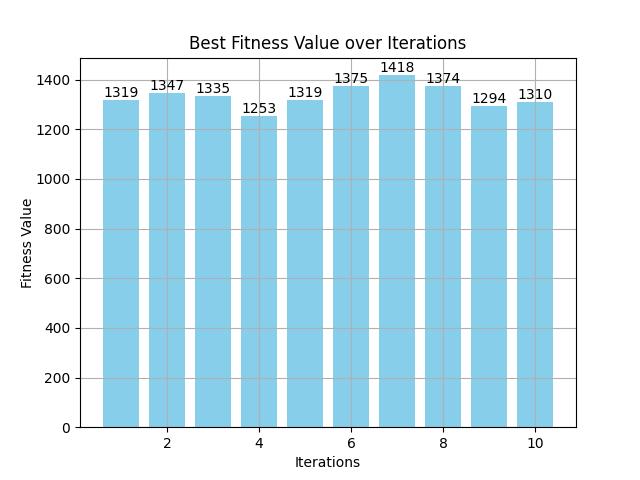
\includegraphics[width=0.5\textwidth]{images/JSSP_rbstr150-40-2000-0.5-10.png}
    \caption{JSSP, Rank-based selection and Truncation, Population Size: 150, Offspring Size: 40, Number of Generations: 2000, Mutation Rate: 0.5, Iterations: 10}
\end{figure}

% The following parameters were used to achieve the result in \textit{Figure 5}:

% \begin{enumerate}
%     \item \textbf{Population Size:} 150
%     \item \textbf{Offspring Size:} 40
%     \item \textbf{Number of Generations:} 2000
%     \item \textbf{Mutation Rate:} 0.5
%     \item \textbf{Iterations:} 10
% \end{enumerate}

\newpage

\subsubsection{Input files ``abz6'' and ``abz7''}

The combination of schemes for both the input files are random and truncation with the following parameters:

\begin{enumerate}
    \item \textbf{Population Size:} 1000
    \item \textbf{Offspring Size:} 200
    \item \textbf{Number of Generations:} 500
    \item \textbf{Mutation Rate:} 0.45
    \item \textbf{Iterations:} 10
\end{enumerate}

The best score for the input file ``abz6'' was \textbf{972}. Whereas, the best score for the input file ``abz7'' was \textbf{776}. The reason for the scores of input file ``abz6'' and ``abd7'' being lower than the input ``abz5'' is due to the fact that the time needed by each process on each machine is significantly low. 

\newpage

\begin{figure}[h]
    \centering
    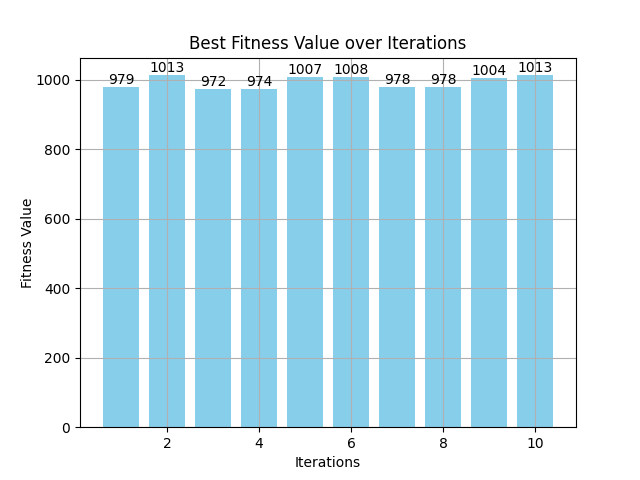
\includegraphics[width=1\textwidth]{images/abz6_rntr1000-200-500-0.45-10.png}
    \caption{Job-shop Scheduling Problem: Input file abz6}
\end{figure}

The following table and graph are generated on the same selection schemes and parameters, except for the fact that the generation size is 25. 

\newpage

\begin{figure}[h]
    \centering
    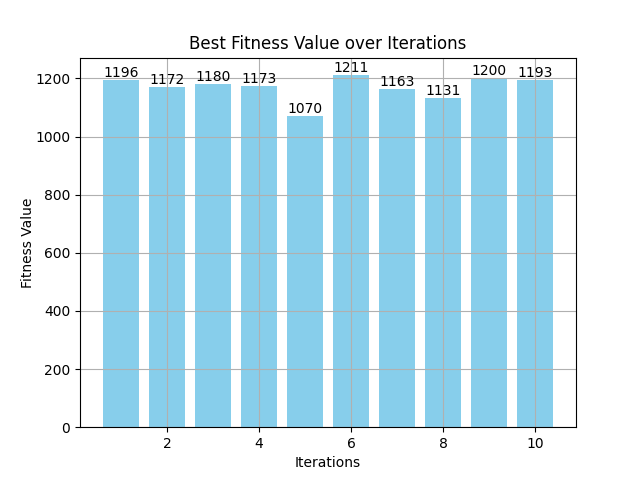
\includegraphics[width=1\textwidth]{images/JSSP_rntrbestscorelessgensABZ6.png}
    \caption{Job-shop Scheduling Problem: Input file abz6 with fewer generations}
\end{figure}

\newpage

\begin{table}[h]
    \centering
    \caption{Generation-wise Best Fitness Scores for Input File \texttt{abz6}}
    \label{tab:best_fitness_scores_abz6}
    \begin{adjustbox}{max width=1\textwidth} % Adjust the table width
        \begin{tabular}{*{12}{c}}
            \toprule
            Generations & Iteration 1 & Iteration 2 & Iteration 3 & Iteration 4 & Iteration 5 & Iteration 6 & Iteration 7 & Iteration 8 & Iteration 9 & Iteration 10 & Best Fitness Score \\
            \midrule
            Gen 1 & 1204 & 1240 & 1279 & 1224 & 1193 & 1288 & 1279 & 1214 & 1264 & 1231 & 1193 \\
            Gen 2 & 1204 & 1240 & 1279 & 1224 & 1193 & 1288 & 1279 & 1214 & 1264 & 1231 & 1193 \\
            Gen 3 & 1204 & 1240 & 1279 & 1224 & 1193 & 1288 & 1279 & 1214 & 1264 & 1231 & 1193 \\
            Gen 4 & 1204 & 1172 & 1279 & 1224 & 1193 & 1288 & 1279 & 1214 & 1264 & 1231 & 1172 \\
            Gen 5 & 1204 & 1172 & 1279 & 1224 & 1193 & 1273 & 1250 & 1214 & 1264 & 1231 & 1172 \\
            Gen 6 & 1204 & 1172 & 1279 & 1224 & 1193 & 1273 & 1250 & 1214 & 1264 & 1231 & 1172 \\
            Gen 7 & 1204 & 1172 & 1279 & 1224 & 1193 & 1273 & 1250 & 1214 & 1252 & 1231 & 1172 \\
            Gen 8 & 1204 & 1172 & 1274 & 1190 & 1193 & 1273 & 1250 & 1176 & 1252 & 1231 & 1172 \\
            Gen 9 & 1204 & 1172 & 1251 & 1190 & 1193 & 1273 & 1250 & 1176 & 1252 & 1231 & 1172 \\
            Gen 10 & 1204 & 1172 & 1251 & 1190 & 1182 & 1273 & 1250 & 1176 & 1252 & 1231 & 1172 \\
            Gen 11 & 1204 & 1172 & 1207 & 1190 & 1182 & 1273 & 1250 & 1176 & 1252 & 1231 & 1172 \\
            Gen 12 & 1204 & 1172 & 1207 & 1190 & 1182 & 1273 & 1250 & 1176 & 1252 & 1231 & 1172 \\
            Gen 13 & 1204 & 1172 & 1180 & 1190 & 1182 & 1273 & 1232 & 1176 & 1252 & 1231 & 1172 \\
            Gen 14 & 1204 & 1172 & 1180 & 1190 & 1182 & 1273 & 1232 & 1176 & 1252 & 1214 & 1172 \\
            Gen 15 & 1204 & 1172 & 1180 & 1190 & 1094 & 1232 & 1232 & 1176 & 1252 & 1214 & 1094 \\
            Gen 16 & 1196 & 1172 & 1180 & 1190 & 1094 & 1232 & 1232 & 1176 & 1252 & 1214 & 1094 \\
            Gen 17 & 1196 & 1172 & 1180 & 1190 & 1094 & 1232 & 1232 & 1176 & 1252 & 1214 & 1094 \\
            Gen 18 & 1196 & 1172 & 1180 & 1190 & 1094 & 1232 & 1232 & 1176 & 1243 & 1214 & 1094 \\
            Gen 19 & 1196 & 1172 & 1180 & 1190 & 1094 & 1232 & 1232 & 1176 & 1243 & 1214 & 1094 \\
            Gen 20 & 1196 & 1172 & 1180 & 1173 & 1094 & 1211 & 1204 & 1176 & 1243 & 1214 & 1094 \\
            Gen 21 & 1196 & 1172 & 1180 & 1173 & 1094 & 1211 & 1204 & 1176 & 1243 & 1214 & 1094 \\
            Gen 22 & 1196 & 1172 & 1180 & 1173 & 1094 & 1211 & 1204 & 1176 & 1219 & 1214 & 1094 \\
            Gen 23 & 1196 & 1172 & 1180 & 1173 & 1094 & 1211 & 1192 & 1176 & 1210 & 1214 & 1094 \\
            Gen 24 & 1196 & 1172 & 1180 & 1173 & 1070 & 1211 & 1192 & 1131 & 1210 & 1214 & 1070 \\
            Gen 25 & 1196 & 1172 & 1180 & 1173 & 1070 & 1211 & 1163 & 1131 & 1200 & 1193 & 1070 \\
            \bottomrule
        \end{tabular}
    \end{adjustbox}
\end{table}

% \newpage

\begin{table}[h]
    \centering
    \caption{Generation-wise Average Fitness Scores for Input File \texttt{abz6}}
    \label{tab:average_fitness_scores_abz6}
    \begin{adjustbox}{max width=1\textwidth} % Adjust the table width
        \begin{tabular}{*{12}{c}}
            \toprule
            Generations & Iteration 1 & Iteration 2 & Iteration 3 & Iteration 4 & Iteration 5 & Iteration 6 & Iteration 7 & Iteration 8 & Iteration 9 & Iteration 10 & Average Fitness Score \\
            \midrule
            Gen 1 & 1204 & 1240 & 1279 & 1224 & 1193 & 1288 & 1279 & 1214 & 1264 & 1231 & 1231.3 \\
            Gen 2 & 1204 & 1240 & 1279 & 1224 & 1193 & 1288 & 1279 & 1214 & 1264 & 1231 & 1231.3 \\
            Gen 3 & 1204 & 1240 & 1279 & 1224 & 1193 & 1288 & 1279 & 1214 & 1264 & 1231 & 1231.3 \\
            Gen 4 & 1204 & 1172 & 1279 & 1224 & 1193 & 1288 & 1279 & 1214 & 1264 & 1231 & 1215.1 \\
            Gen 5 & 1204 & 1172 & 1279 & 1224 & 1193 & 1273 & 1250 & 1214 & 1264 & 1231 & 1213.1 \\
            Gen 6 & 1204 & 1172 & 1279 & 1224 & 1193 & 1273 & 1250 & 1214 & 1264 & 1231 & 1213.1 \\
            Gen 7 & 1204 & 1172 & 1279 & 1224 & 1193 & 1273 & 1250 & 1214 & 1252 & 1231 & 1210.6 \\
            Gen 8 & 1204 & 1172 & 1274 & 1190 & 1193 & 1273 & 1250 & 1176 & 1252 & 1231 & 1199.6 \\
            Gen 9 & 1204 & 1172 & 1251 & 1190 & 1193 & 1273 & 1250 & 1176 & 1252 & 1231 & 1199.6 \\
            Gen 10 & 1204 & 1172 & 1251 & 1190 & 1182 & 1273 & 1250 & 1176 & 1252 & 1231 & 1197.6 \\
            Gen 11 & 1204 & 1172 & 1207 & 1190 & 1182 & 1273 & 1250 & 1176 & 1252 & 1231 & 1195.6 \\
            Gen 12 & 1204 & 1172 & 1207 & 1190 & 1182 & 1273 & 1250 & 1176 & 1252 & 1231 & 1195.6 \\
            Gen 13 & 1204 & 1172 & 1180 & 1190 & 1182 & 1273 & 1232 & 1176 & 1252 & 1231 & 1192.5 \\
            Gen 14 & 1204 & 1172 & 1180 & 1190 & 1182 & 1273 & 1232 & 1176 & 1252 & 1214 & 1191.8 \\
            Gen 15 & 1204 & 1172 & 1180 & 1190 & 1094 & 1232 & 1232 & 1176 & 1252 & 1214 & 1179.6 \\
            Gen 16 & 1196 & 1172 & 1180 & 1190 & 1094 & 1232 & 1232 & 1176 & 1252 & 1214 & 1179.4 \\
            Gen 17 & 1196 & 1172 & 1180 & 1190 & 1094 & 1232 & 1232 & 1176 & 1252 & 1214 & 1179.4 \\
            Gen 18 & 1196 & 1172 & 1180 & 1190 & 1094 & 1232 & 1232 & 1176 & 1243 & 1214 & 1176.4 \\
            Gen 19 & 1196 & 1172 & 1180 & 1190 & 1094 & 1232 & 1232 & 1176 & 1243 & 1214 & 1176.4 \\
            Gen 20 & 1196 & 1172 & 1180 & 1173 & 1094 & 1211 & 1204 & 1176 & 1243 & 1214 & 1173.4 \\
            Gen 21 & 1196 & 1172 & 1180 & 1173 & 1094 & 1211 & 1204 & 1176 & 1243 & 1214 & 1173.4 \\
            Gen 22 & 1196 & 1172 & 1180 & 1173 & 1094 & 1211 & 1204 & 1176 & 1219 & 1214 & 1171.9 \\
            Gen 23 & 1196 & 1172 & 1180 & 1173 & 1094 & 1211 & 1192 & 1176 & 1210 & 1214 & 1168.8 \\
            Gen 24 & 1196 & 1172 & 1180 & 1173 & 1070 & 1211 & 1192 & 1131 & 1210 & 1214 & 1163.6 \\
            Gen 25 & 1196 & 1172 & 1180 & 1173 & 1070 & 1211 & 1163 & 1131 & 1200 & 1193 & 1155.6 \\
            \bottomrule
        \end{tabular}
    \end{adjustbox}
\end{table}

\newpage

\begin{figure}[h]
    \centering
    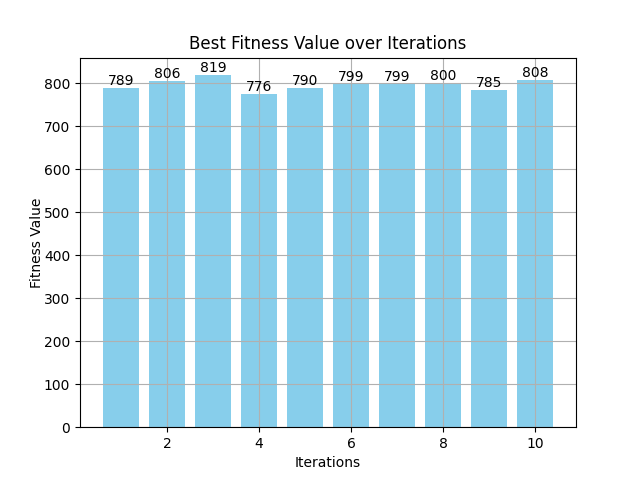
\includegraphics[width=1\textwidth]{images/abz7_rntr1000-200-500-0.45-10.png}
    \caption{Job-shop Scheduling Problem: Input file abz7}
\end{figure}

\newpage

\begin{figure}[h]
    \centering
    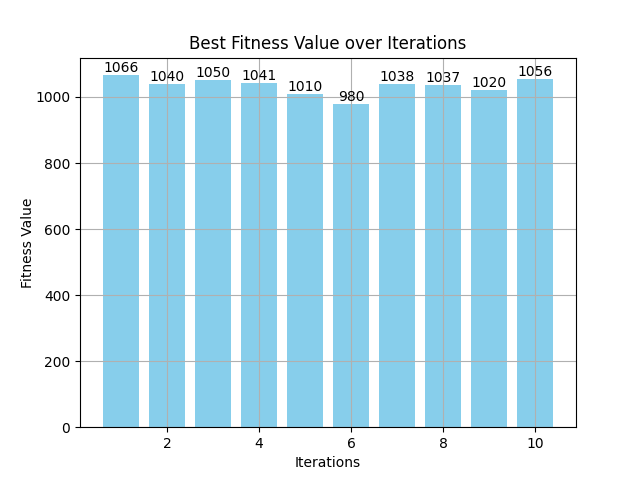
\includegraphics[width=1\textwidth]{images/JSSP_rntrbestscorelessgensABZ7.png}
    \caption{Job-shop Scheduling Problem: Input file abz7 with 25 generations}
\end{figure}

\newpage

\begin{table}[h]
    \centering
    \caption{Generation-wise Fitness Scores for Input File \texttt{abz7}}
    \label{tab:fitness_scores_abz6}
    \begin{adjustbox}{max width=1\textwidth} % Adjust the table width
        \begin{tabular}{*{12}{c}}
            \toprule
            Generations & Iteration 1 & Iteration 2 & Iteration 3 & Iteration 4 & Iteration 5 & Iteration 6 & Iteration 7 & Iteration 8 & Iteration 9 & Iteration 10 & Best Fitness Score \\
            \midrule
            Gen 1 & 1102 & 1081 & 1067 & 1053 & 1049 & 980 & 1092 & 1067 & 1061 & 1097 & 980 \\
            Gen 2 & 1102 & 1081 & 1067 & 1053 & 1049 & 980 & 1092 & 1067 & 1061 & 1097 & 980 \\
            Gen 3 & 1102 & 1081 & 1067 & 1053 & 1049 & 980 & 1038 & 1067 & 1061 & 1097 & 980 \\
            Gen 4 & 1102 & 1081 & 1050 & 1053 & 1049 & 980 & 1038 & 1067 & 1061 & 1097 & 980 \\
            Gen 5 & 1099 & 1081 & 1050 & 1053 & 1049 & 980 & 1038 & 1067 & 1061 & 1097 & 980 \\
            Gen 6 & 1099 & 1081 & 1050 & 1053 & 1049 & 980 & 1038 & 1067 & 1061 & 1097 & 980 \\
            Gen 7 & 1099 & 1081 & 1050 & 1053 & 1049 & 980 & 1038 & 1067 & 1061 & 1097 & 980 \\
            Gen 8 & 1099 & 1081 & 1050 & 1053 & 1049 & 980 & 1038 & 1067 & 1061 & 1097 & 980 \\
            Gen 9 & 1098 & 1081 & 1050 & 1053 & 1049 & 980 & 1038 & 1067 & 1061 & 1097 & 980 \\
            Gen 10 & 1066 & 1081 & 1050 & 1053 & 1049 & 980 & 1038 & 1067 & 1061 & 1097 & 980 \\
            Gen 11 & 1066 & 1081 & 1050 & 1053 & 1049 & 980 & 1038 & 1067 & 1061 & 1097 & 980 \\
            Gen 12 & 1066 & 1081 & 1050 & 1053 & 1049 & 980 & 1038 & 1067 & 1061 & 1097 & 980 \\
            Gen 13 & 1066 & 1081 & 1050 & 1053 & 1049 & 980 & 1038 & 1067 & 1061 & 1097 & 980 \\
            Gen 14 & 1066 & 1081 & 1050 & 1053 & 1010 & 980 & 1038 & 1067 & 1061 & 1080 & 980 \\
            Gen 15 & 1066 & 1081 & 1050 & 1053 & 1010 & 980 & 1038 & 1067 & 1061 & 1070 & 980 \\
            Gen 16 & 1066 & 1081 & 1050 & 1053 & 1010 & 980 & 1038 & 1067 & 1061 & 1070 & 980 \\
            Gen 17 & 1066 & 1081 & 1050 & 1053 & 1010 & 980 & 1038 & 1067 & 1061 & 1070 & 980 \\
            Gen 18 & 1066 & 1081 & 1050 & 1053 & 1010 & 980 & 1038 & 1067 & 1061 & 1070 & 980 \\
            Gen 19 & 1066 & 1063 & 1050 & 1053 & 1010 & 980 & 1038 & 1067 & 1061 & 1070 & 980 \\
            Gen 20 & 1066 & 1040 & 1050 & 1053 & 1010 & 980 & 1038 & 1067 & 1061 & 1070 & 980 \\
            Gen 21 & 1066 & 1040 & 1050 & 1053 & 1010 & 980 & 1038 & 1067 & 1061 & 1070 & 980 \\
            Gen 22 & 1066 & 1040 & 1050 & 1044 & 1010 & 980 & 1038 & 1067 & 1061 & 1070 & 980 \\
            Gen 23 & 1066 & 1040 & 1050 & 1044 & 1010 & 980 & 1038 & 1067 & 1061 & 1056 & 980 \\
            Gen 24 & 1066 & 1040 & 1050 & 1041 & 1010 & 980 & 1038 & 1067 & 1061 & 1056 & 980 \\
            Gen 25 & 1066 & 1040 & 1050 & 1041 & 1010 & 980 & 1038 & 1065 & 1020 & 1056 & 980 \\
            \bottomrule
        \end{tabular}
    \end{adjustbox}
\end{table}

% \newpage

\begin{table}[h]
    \centering
    \caption{Generation-wise Average Fitness Scores for Input File \texttt{abz7}}
    \label{tab:average_fitness_scores_abz6}
    \begin{adjustbox}{max width=1\textwidth} % Adjust the table width
        \begin{tabular}{*{12}{c}}
            \toprule
            Generations & Iteration 1 & Iteration 2 & Iteration 3 & Iteration 4 & Iteration 5 & Iteration 6 & Iteration 7 & Iteration 8 & Iteration 9 & Iteration 10 & Average Fitness Score \\
            \midrule
            Gen 1 & 1102 & 1081 & 1067 & 1053 & 1049 & 980 & 1092 & 1067 & 1061 & 1097 & 1051.9 \\
            Gen 2 & 1102 & 1081 & 1067 & 1053 & 1049 & 980 & 1092 & 1067 & 1061 & 1097 & 1051.9 \\
            Gen 3 & 1102 & 1081 & 1067 & 1053 & 1049 & 980 & 1038 & 1067 & 1061 & 1097 & 1052.5 \\
            Gen 4 & 1102 & 1081 & 1050 & 1053 & 1049 & 980 & 1038 & 1067 & 1061 & 1097 & 1048.8 \\
            Gen 5 & 1099 & 1081 & 1050 & 1053 & 1049 & 980 & 1038 & 1067 & 1061 & 1097 & 1049.5 \\
            Gen 6 & 1099 & 1081 & 1050 & 1053 & 1049 & 980 & 1038 & 1067 & 1061 & 1097 & 1049.5 \\
            Gen 7 & 1099 & 1081 & 1050 & 1053 & 1049 & 980 & 1038 & 1067 & 1061 & 1097 & 1049.5 \\
            Gen 8 & 1099 & 1081 & 1050 & 1053 & 1049 & 980 & 1038 & 1067 & 1061 & 1097 & 1049.5 \\
            Gen 9 & 1098 & 1081 & 1050 & 1053 & 1049 & 980 & 1038 & 1067 & 1061 & 1097 & 1049.4 \\
            Gen 10 & 1066 & 1081 & 1050 & 1053 & 1049 & 980 & 1038 & 1067 & 1061 & 1097 & 1047.2 \\
            Gen 11 & 1066 & 1081 & 1050 & 1053 & 1049 & 980 & 1038 & 1067 & 1061 & 1097 & 1047.2 \\
            Gen 12 & 1066 & 1081 & 1050 & 1053 & 1049 & 980 & 1038 & 1067 & 1061 & 1097 & 1047.2 \\
            Gen 13 & 1066 & 1081 & 1050 & 1053 & 1049 & 980 & 1038 & 1067 & 1061 & 1097 & 1047.2 \\
            Gen 14 & 1066 & 1081 & 1050 & 1053 & 1010 & 980 & 1038 & 1067 & 1061 & 1080 & 1046.8 \\
            Gen 15 & 1066 & 1081 & 1050 & 1053 & 1010 & 980 & 1038 & 1067 & 1061 & 1070 & 1045.6 \\
            Gen 16 & 1066 & 1081 & 1050 & 1053 & 1010 & 980 & 1038 & 1067 & 1061 & 1070 & 1045.6 \\
            Gen 17 & 1066 & 1081 & 1050 & 1053 & 1010 & 980 & 1038 & 1067 & 1061 & 1070 & 1045.6 \\
            Gen 18 & 1066 & 1081 & 1050 & 1053 & 1010 & 980 & 1038 & 1067 & 1061 & 1070 & 1045.6 \\
            Gen 19 & 1066 & 1063 & 1050 & 1053 & 1010 & 980 & 1038 & 1067 & 1061 & 1070 & 1044.8 \\
            Gen 20 & 1066 & 1040 & 1050 & 1053 & 1010 & 980 & 1038 & 1067 & 1061 & 1070 & 1043.5 \\
            Gen 21 & 1066 & 1040 & 1050 & 1053 & 1010 & 980 & 1038 & 1067 & 1061 & 1070 & 1043.5 \\
            Gen 22 & 1066 & 1040 & 1050 & 1044 & 1010 & 980 & 1038 & 1067 & 1061 & 1070 & 1042.4 \\
            Gen 23 & 1066 & 1040 & 1050 & 1044 & 1010 & 980 & 1038 & 1067 & 1061 & 1056 & 1040.4 \\
            Gen 24 & 1066 & 1040 & 1050 & 1041 & 1010 & 980 & 1038 & 1067 & 1061 & 1056 & 1039.6 \\
            Gen 25 & 1066 & 1040 & 1050 & 1041 & 1010 & 980 & 1038 & 1065 & 1020 & 1056 & 1039.0 \\
            \bottomrule
        \end{tabular}
    \end{adjustbox}
\end{table}

\newpage

\section{Evolutionary Art: Mona Lisa}

\subsection{Problem Formulation}

Our chromosome follows a similar pattern to the previously mentioned ones. Each chromosome is a tuple with the first index containing the actual chromosome and the second index storing its fitness value. The main chromosome itself is a list of \( n \) polygons, \( P \). In our case, \( n = 50 \), and each polygon \( P \) is represented in the following form as a Python dictionary:

\[
P: \{ x: [x_1, x_2, x_3],\, y: [y_1, y_2, y_3],\, color: (R, G, B, A) \}
\]

Since each polygon is a triangle, we need 3 \( x \) and \( y \) values to represent them and a fill color in the RGBA form.

For crossover, we are simply generating a random crossover point and splitting the parents list there. Each offspring takes an alternate half of the parents.
Offspring A takes the first half of parent A and second half of parent B and vice versa for Offspring B.
These halves are generated by dissecting the list according to the generated crossover point

Our idea of mutation is to modify a single polygon inside the chromosome which comprises n polygons. 
For this, we simply remove the last triangle by popping from the list and then add a randomly generated polygon in order to mutate the chromosome.
\subsection{Analysis}

\begin{figure}[h]
    \centering
    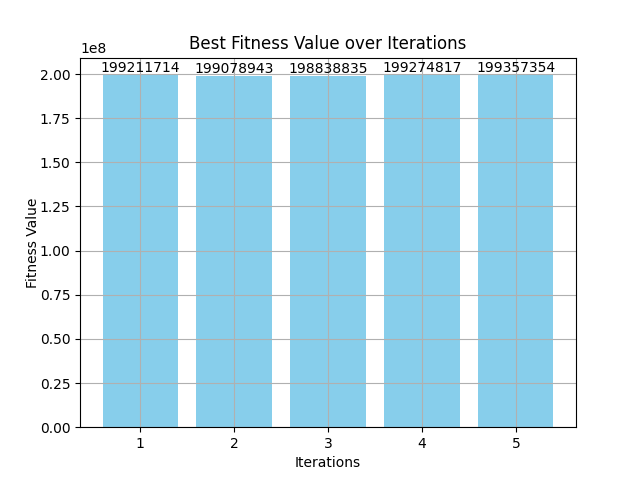
\includegraphics[width=0.5\textwidth]{images/MonaLisa graph.png}
    \caption{Evolutionary art Mona Lisa}
\end{figure}

\newpage

\begin{figure}[h]
    \centering
    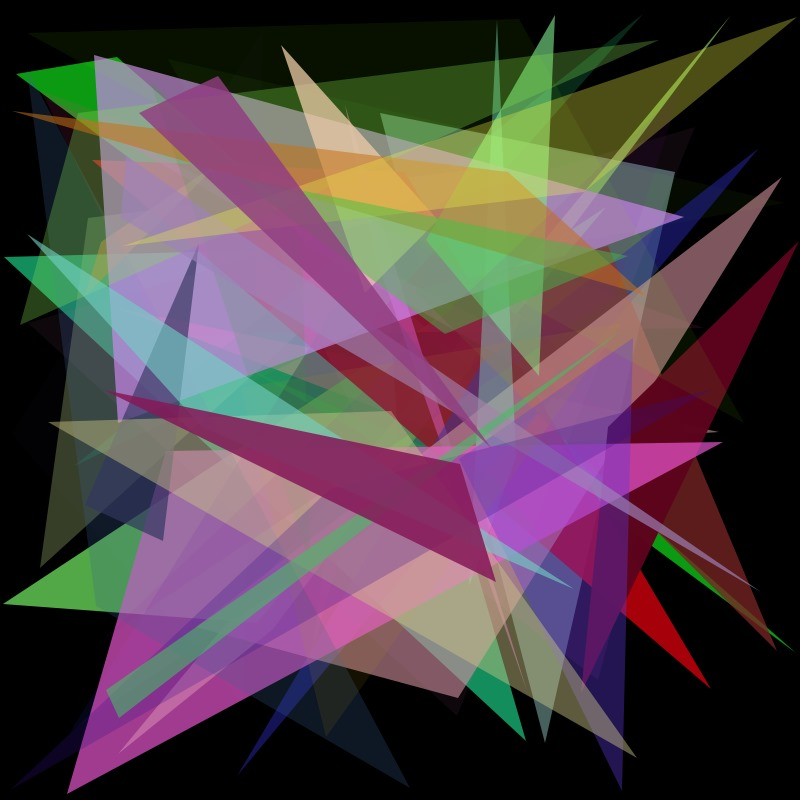
\includegraphics[width=1\textwidth]{images/Monagen1.jpg}
    \caption{Evolutionary art Mona Lisa: First Generation of Mona Lisa}
\end{figure}

\newpage

\begin{figure}[h]
    \centering
    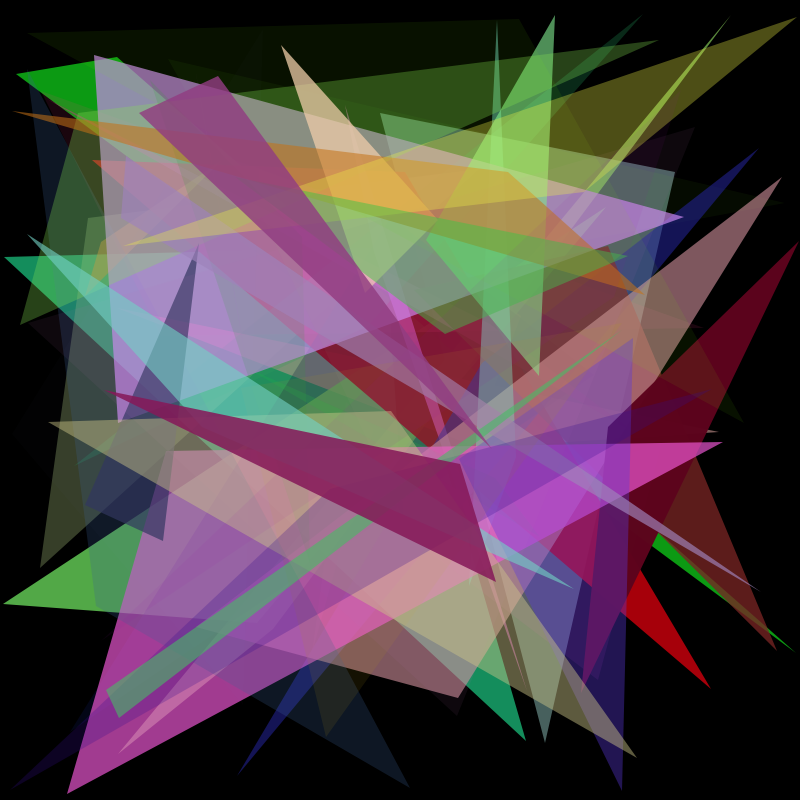
\includegraphics[width=1\textwidth]{gen_mona.png}
    \caption{Evolutionary art Mona Lisa: 50th Generation of Mona Lisa}
\end{figure}

\newpage

\section{Discussion and General Analysis}

In all the problems, we noticed the trend that exploitative methods worked better as survival selection schemes while explorative fared better as parent selection schemes. This is the reason why we largely kept truncation as our survival selector.
\newline \\
Looking at our scores, we can probably conclude that even though it does provide good scores in earlier generations it is possible to reach a local maxima quickly through this approach. This is down to the fact that our survival selection is truncation and as a result the tradeoff is while we get better scores quicker, the possibility of hitting local minimas are very high. 
\newline \\
We mostly used tried working with random, rank-based selection, or binary tournament selection as our parent selection schemes to balance out the exploitative nature of truncation. The opposite ends of the spectrum that two of our selection schemes provided proved to work well for us. 
\newline \\
However, it was interesting to notice how a selection scheme used for both parent and survival selection did not work well. While this is obvious in the case of using random, or truncation as both parent and survival schemes. It was interesting to see how none of the schemes when used twice were giving great results. Discussing this we realized that every selection scheme inherently lies either towards the exploitative side or the explorative side, and for an evolutionary alogrithm, ideally the sweet spot should be equal exploitative and explorative. This is why a combination of two different schemes worked better always. 
\newline \\
While trying to improve our scores, we also slightly noticed a pattern between keep a specific ratio between population, offspring size, and mutation rate. We noticed a higher population size with a ratio of 5:1 or 4:1 to offpsring size is a good spot, while keeping the mutation rate at a moderate central level of 0.5 or 0.45.

\end{document}